\graphicspath{{images/}}

\section{Методы решения обыкновенных дифференциальных уравнений}

\subsection{Решение задачи Коши для ОДУ}

\subsubsection{Постановка задачи}
Реализовать методы Эйлера, Рунге-Кутты и Адамса 4-го порядка в виде программ, задавая в качестве входных данных шаг сетки $h$. С использованием разработанного программного обеспечения решить задачу Коши для ОДУ 2-го порядка на указанном отрезке. Оценить погрешность численного решения с использованием метода Рунге-Ромберга и путем сравнения с точным решением.

\subsubsection{Консоль}
\begin{alltt}
1 2
2 1 0.1
Метод Эйлера:
x = [1.000000, 1.100000, 1.200000, 1.300000, 1.400000, 1.500000, 1.600000, 1.700000, 1.800000, 1.900000, 2.000000]
y = [2.000000, 2.100000, 2.440000, 2.988264, 3.739862, 4.703645, 5.896398, 7.340012, 9.060020, 11.084804, 13.445144]
Погрешность вычислений:
1.188858
Метод Рунге-Кутты:
x = [1.000000, 1.100000, 1.200000, 1.300000, 1.400000, 1.500000, 1.600000, 1.700000, 1.800000, 1.900000, 2.000000]
y = [2.000000, 2.215465, 2.652360, 3.311306, 4.206041, 5.358762, 6.797651, 8.555485, 10.668830, 13.177560, 16.124554]
Погрешность вычислений:
0.000027
Метод Адамса:
x = [1.000000, 1.100000, 1.200000, 1.300000, 1.400000, 1.500000, 1.600000, 1.700000, 1.800000, 1.900000, 2.000000]
y = [2.000000, 2.215465, 2.652360, 3.311306, 4.205356, 5.357862, 6.796735, 8.554608, 10.668022, 13.176829, 16.123898]
Погрешность вычислений:
0.000074
\end{alltt}
\pagebreak

\subsubsection{Результат}
Метод Эйлера
\begin{center}
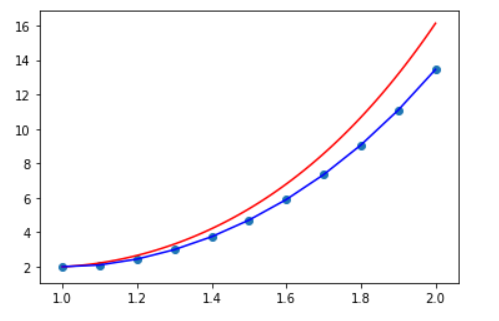
\includegraphics[scale=0.75]{4-1euler}
\end{center}

Метод Рунге-Кутты
\begin{center}
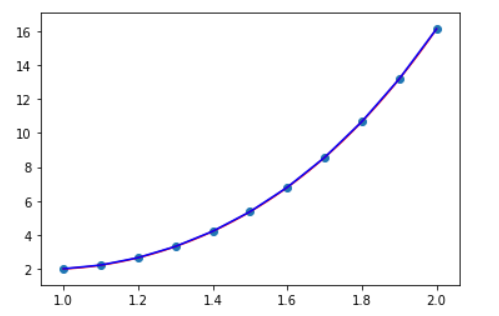
\includegraphics[scale=0.75]{4-1runge}
\end{center}
\pagebreak

Метод Адамса
\begin{center}
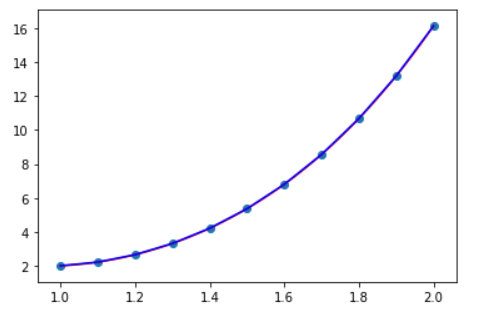
\includegraphics[scale=0.75]{4-1adams}
\end{center}
\pagebreak

\subsubsection{Исходный код}
\lstinputlisting{../../NM4_1/desolve.h}
\pagebreak

\subsection{Решение краевых задач}

\subsubsection{Постановка задачи}
Реализовать метод стрельбы и конечно-разностный метод решения краевой задачи для ОДУ в виде программ. С использованием разработанного программного обеспечения решить краевую задачу для обыкновенного дифференциального уравнения 2-го порядка на указанном отрезке. Оценить погрешность численного решения с использованием метода Рунге-Ромберга и путем сравнения с точным решением.

\subsubsection{Консоль}
\begin{alltt}
0.1 0.00001
Метод стрельбы:
x = [1.000000, 1.100000, 1.200000, 1.300000, 1.400000, 1.500000, 1.600000, 1.700000, 1.800000, 1.900000, 2.000000]
y = [2.718310, 3.635057, 4.780968, 6.201090, 7.948142, 10.083714, 12.679630, 15.819517, 19.600595, 24.135726, 29.555762]
Погрешность вычислений:
0.000029
Конечно-разностный метод:
x = [1.000000, 1.100000, 1.200000, 1.300000, 1.400000, 1.500000, 1.600000, 1.700000, 1.800000, 1.900000, 2.000000]
y = [1.171219, 1.986704, 3.035416, 4.365472, 6.033397, 8.105462, 10.659212, 13.785218, 17.589089, 22.193780, 27.742225]
Погрешность вычислений:
0.342752
\end{alltt}
\pagebreak

\subsubsection{Результат}
Метод стрельбы
\begin{center}
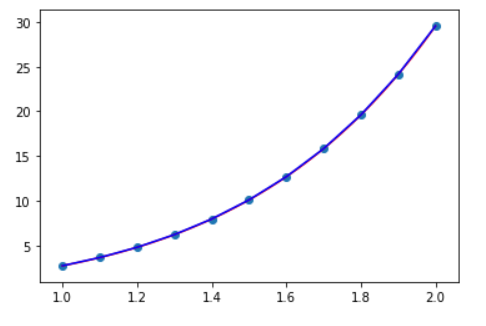
\includegraphics[scale=0.75]{4-2shooting}
\end{center}

Конечно-разностный метод
\begin{center}
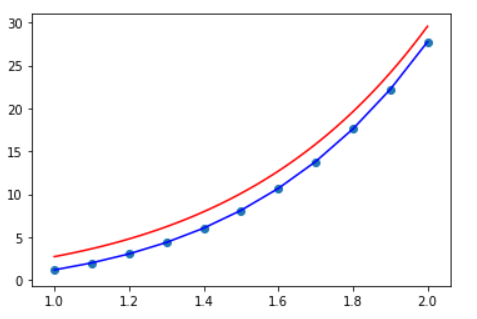
\includegraphics[scale=0.75]{4-2fin-dif}
\end{center}
\pagebreak

\subsubsection{Исходный код}
\lstinputlisting{../../NM4_2/solver.h}
\pagebreak
